

\documentclass{beamer}


\usepackage[utf8]{inputenc}
\usepackage[T1]{fontenc}
\usepackage{fontawesome}
\usepackage{wrapfig}
\usepackage{tikzsymbols}
\usepackage{hyperref}
\usepackage{enumitem}
 
  
\usetheme{Madrid}

\title{Le Taj Mahal : Histoire et Architecture}

% A subtitle is optional and this may be deleted
%\subtitle{Optional Subtitle}

\author{Arif Ahmed  }
% - Give the names in the same order as the appear in the paper.
% - Use the \inst{?} command only if the authors have different
%   affiliation.

\institute[Université Rennes 2] % (optional, but mostly needed)
{
   CIREFE Soutien Linguistique - A1 \\
  Université Rennes 2 }
  

\date{Avril, 2018}
 
\subject{Introduction}
 

\begin{document}

\begin{frame}
  \titlepage
\end{frame}

\begin{frame}{Le Taj Mahal :   Monument historique}


\begin{figure}[h]
% Replace with a new gorgeous photo
    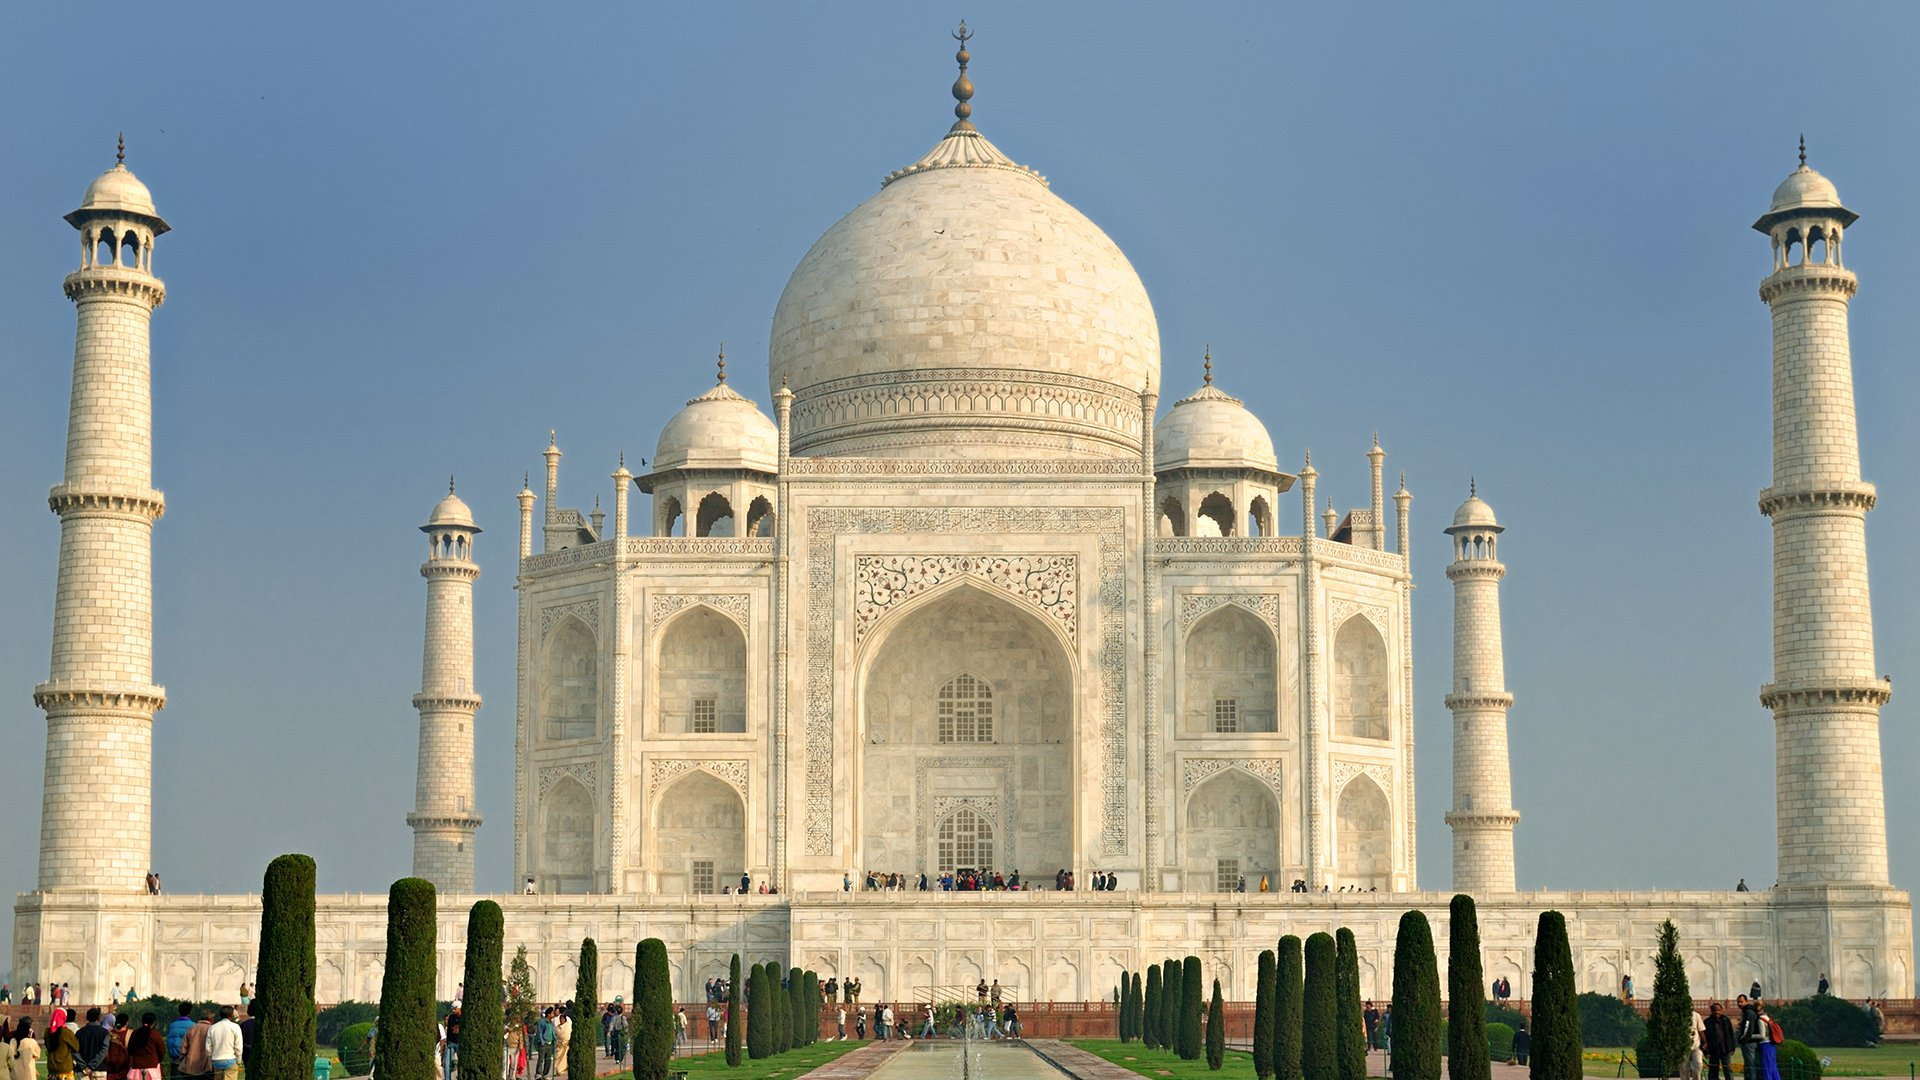
\includegraphics[width=0.88\textwidth]{Taj-Mahal-Grand.jpg}
\end{figure}
\begin{center}
\LARGE C'est magnifique    
\includegraphics[width=0.05\textwidth]{smiling-face-with-heart-eyes.png}
\includegraphics[width=0.05\textwidth]{smiling-face-with-heart-eyes.png}
\includegraphics[width=0.05\textwidth]{smiling-face-with-heart-eyes.png}?
\end{center}
\end{frame}




\begin{frame}{Introduction}
\begin{itemize}[label=$\ast$]

    \item Le Taj Mahal est un \textcolor{green}{mausolée} de marbre [marble] blanc construit par l'empereur moghol \textbf{Shâh Jahân}.
    \item  En mémoire de son épouse \textbf{Mumtaj Begum} 
\includegraphics[width=0.05\textwidth]{heart-balloon-smiley.png}.
    \item  Il est situé sur sud de la rivière Yamuna à Agra.
\end{itemize}

%\begin{figure}[h]
% Figure should include two king + queen
  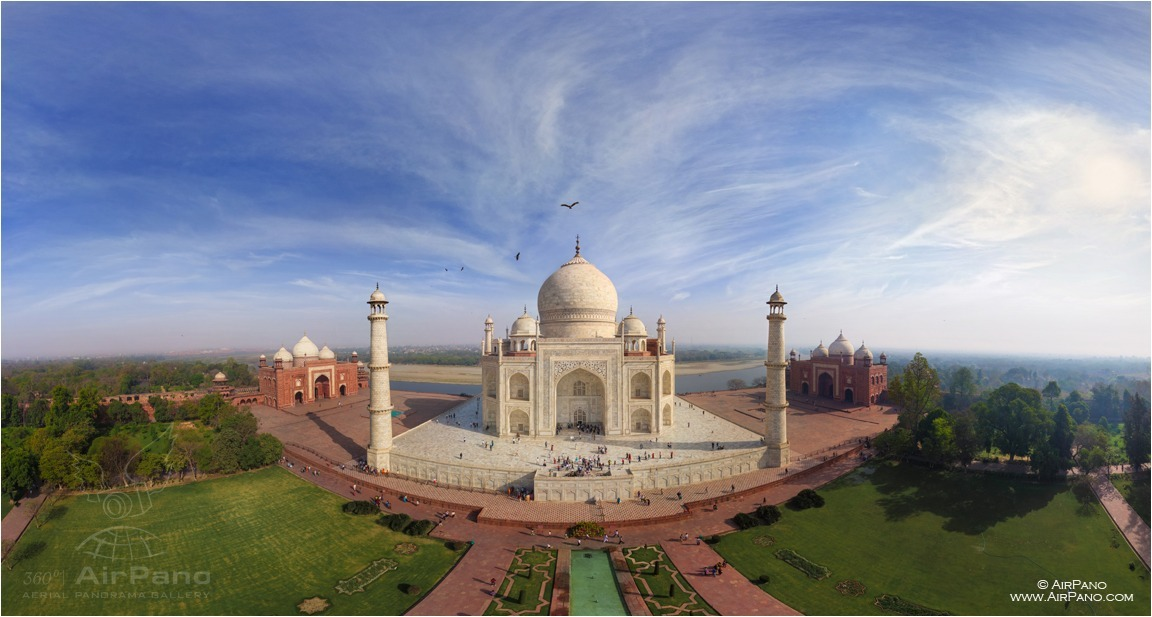
\includegraphics[width=0.45\textwidth]{tajmahal-drone1.jpg}  \quad \quad \quad   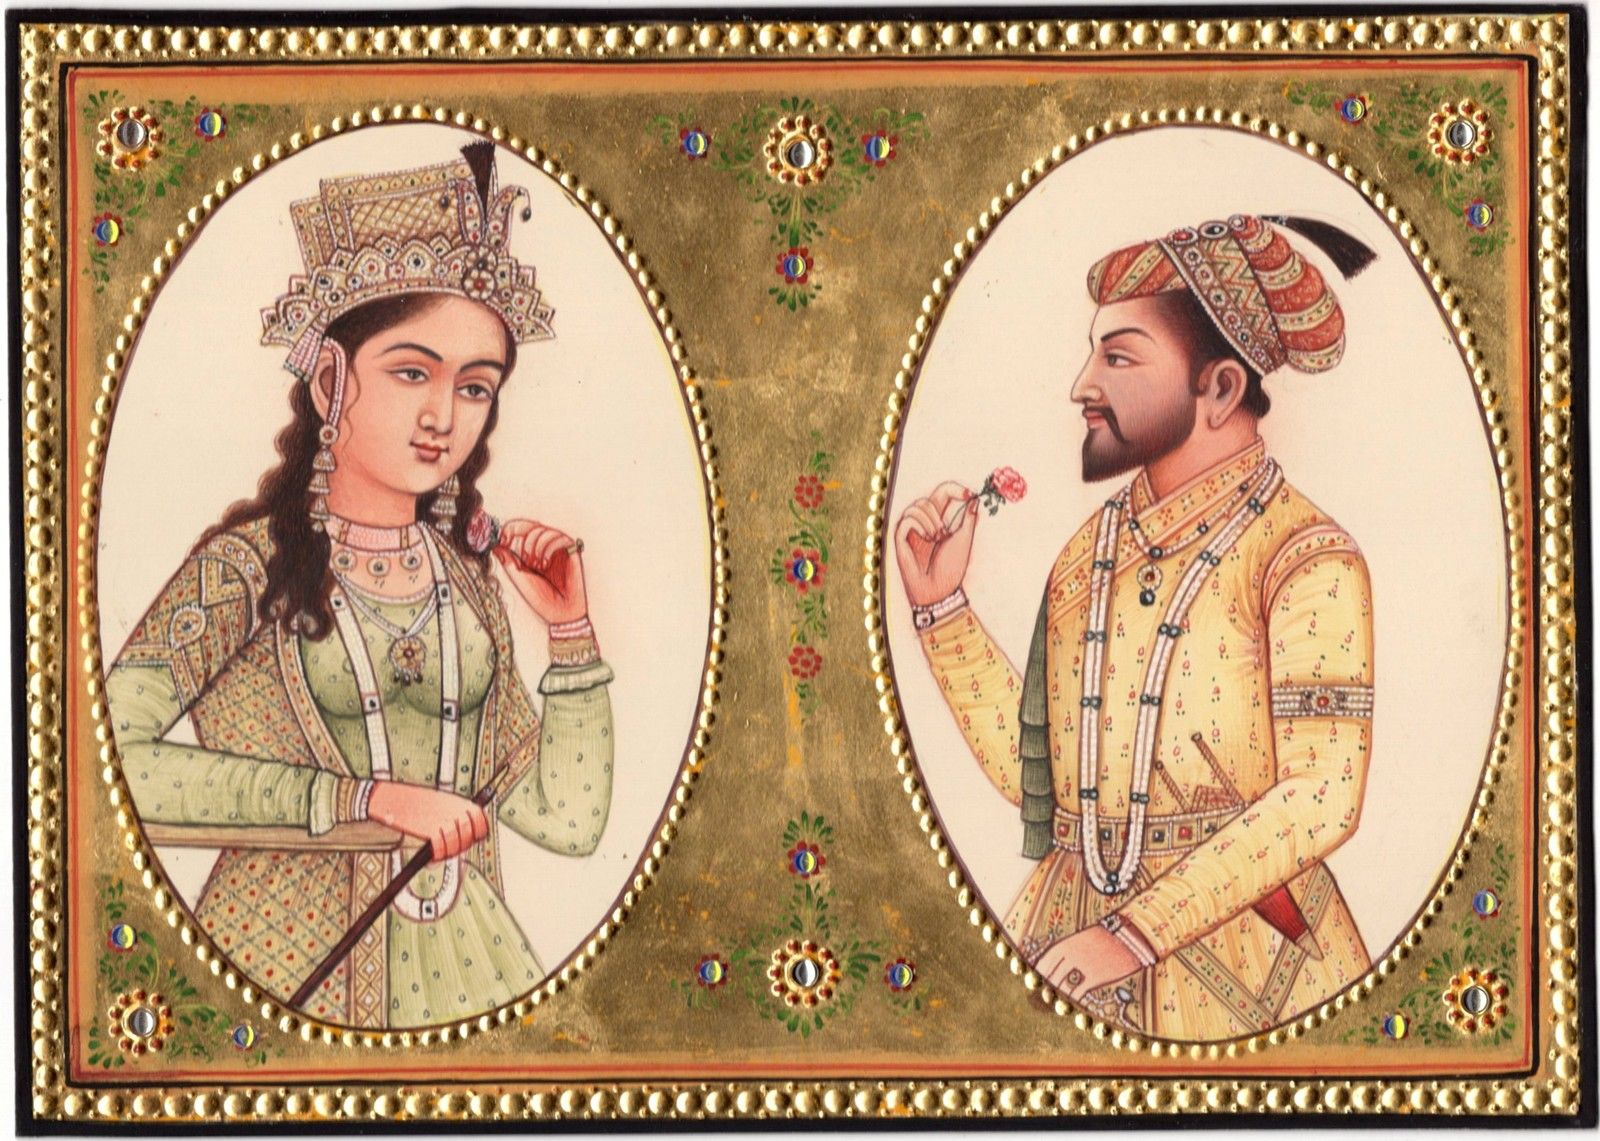
\includegraphics[width=0.35\textwidth]{tajmahal-S-M.jpg}  
  
  
  %\end{figure}

\begin{itemize}
    \item[$\rightarrow$] La construction a commencé en 1632(Apr. J-C) et  terminée en 1648(Apr. J-C).
    \item[$\rightarrow$] Il est considéré comme un joyau [jewel] de \textcolor{red}{l'architecture moghole}.
    \item[$\rightarrow$] Un style qui combine des éléments architecturaux provenant des architectures \textcolor{blue}{\textit{islamique}} et \textcolor{blue}{\textit{indienne}}.
    %\item un style qui combine des éléments architecturaux des architectures islamique, iranienne, ottomane et indienne.
\end{itemize}
 
\end{frame}
 
 
 
 
 
 \begin{frame}{Localisation du Le Taj Mahal}
% Figure should include major indian cities + Taj Mahal

\begin{itemize}
    \item Le Taj Mahal est situé dans le \textbf{nord} de l'Inde, dans l'État \textbf{d'Uttar Pradesh}.
\end{itemize}
 \begin{figure}[h]
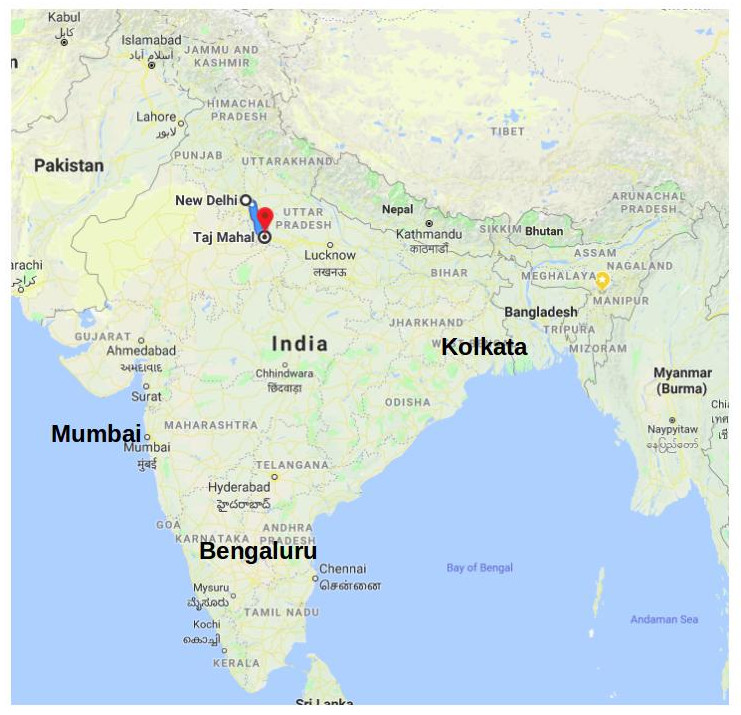
\includegraphics[ [width=0.25\textwidth, scale=0.35]{2018-04-04-21-30-17_Taj-Mahal_3.jpg}
\end{figure}
\end{frame}
 
 
 

\begin{frame}{Comment se rendre au Taj Mahal???}
\begin{itemize}[label=$\ast$]
    \item L'aéroport international \faPlane \hspace{0.2cm}  le plus proche est à New Delhi.
    \item Vous pouvez prendre l'avion pour \textbf{New Delhi}.
\end{itemize}
% Figure should highlight major cities including airport symbol and transport
\begin{figure}[h]
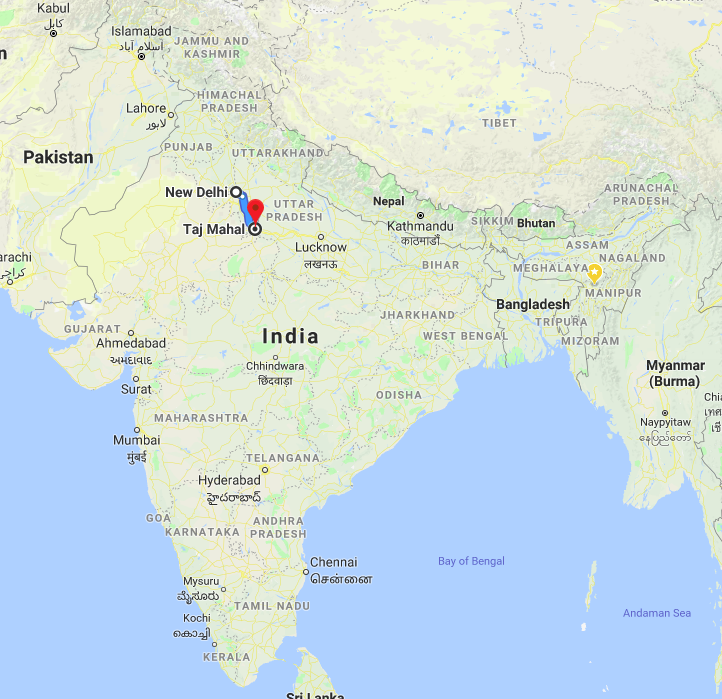
\includegraphics[[width=0.25\textwidth, scale=0.15]{2018-04-04-21-30-17_Taj-Mahal.png}
\end{figure}
 
 \begin{itemize}[label=$\ast$]
     \item Ensuit, Prendre le bus(2h) \faBus \hspace{0.2cm} ou la voiture \faCar  \hspace{0.2cm} ou le train(2h) \faTrain \hspace{0.2cm} de New Delhi (204km).
     \item Vous arrivez au Taj Mahal
\includegraphics[width=0.1\textwidth]{smiley-great-job.jpg}
\end{itemize}
\end{frame}
 
 
 
 
 
% Taj-Mahal-Petit-Arch1
\begin{frame}{Carte de le Taj Mahal}
\begin{figure}[h]
   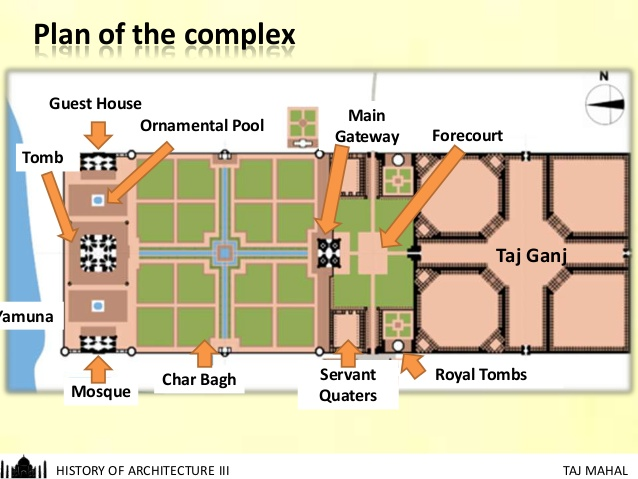
\includegraphics[[width=0.25\textwidth, scale=0.3]{tajmahal-4-638.jpg}
\end{figure}
\tiny {Note : Tomb -> 	la Tombe, Mosque -> la Mosquée, Guest House -> la maison des invités, Pool -> Piscine, Char Bagh -> Le Jardin, Main Gateway -> la porte \\

Forecourt \\  
Taj Ganj \\
}

\footnotetext{\url{https://www.slideshare.net/mumal1992/tajmahal-27131343}}


\end{frame}
 



  
 
 % Taj-Mahal-Petit-Arch1
\begin{frame}{Certaines Des Architectures Importantes(Videos)}



Youtube video 1 : \href{https://www.youtube.com/watch?v=6YZRjSdacqI}{https://www.youtube.com/watch?v=6YZRjSdacqI}

Youtube video 2 : \href{https://www.youtube.com/watch?v=FrIewI8bh2E}{https://www.youtube.com/watch?v=FrIewI8bh2E}

\begin{figure}
\centering

\includegraphics[width=0.25\textwidth]{SmileyMerci.jpg}
\end{figure}

% The Dome
%The Tomb
% The callicgraphy
% Minaretes
% Mosques


% End with the name of the two architectures


\end{frame}
 
 







\end{document}


